\chapter{Alberi ricoprenti minimi}
Gli alberi ricoprenti minimi sono dei particolari alberi per cui, a partire da un grafo non orientato connesso $G=(V,E)$ e una funzione peso $w:E\xrightarrow{}R$, restituisce un albero $T=(V,E')$ con $E' \subseteq E$ tale che per ogni altro albero $T_1 = (V, E'_1)$ si abbia che 
\[w(T) = \sum_{e\in E'} w(e) \leq \sum_{e\in E} w(e) = w(T_1)\]
Cioè, tutti i nodi devono essere connessi e gli archi che li collegano devono avere costo minimo rispetto a tutti gli altri possibili collegamenti.

Naturalmente, il nostro obiettivo sarà quello di non effettuare una ricerca esaustiva poiché questa ha un costo su n vertici di $n^{n-2}$, cioè, un costo esponenziale. 
\section{Taglio e Colorazione}
Sia $G=(V,E)$ un grafo non orientato e connesso con funzione peso $w : E \rightarrow R$, definiamo un \textbf{taglio} di G, una partizione $(V_1,V_2)$ di V non banale. Un arco $(u,v)$ tale che $u\in V_1, v\in V_2$ si dice che \textbf{attraversa il taglio}.
\begin{figure}[H]
    \centering
    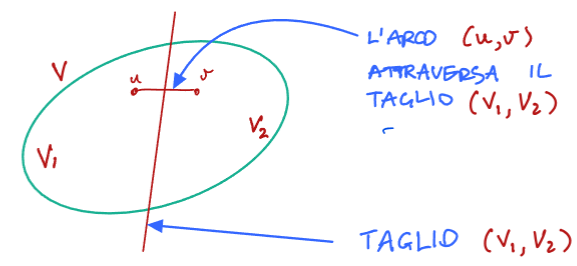
\includegraphics[width=0.6\linewidth]{Images/alberi_cammini_minimi/taglio.png}
\end{figure}
Faremo utilizzo di un \textbf{processo di colorazione}, per cui, finché possibile applicheremo i seguenti passi:
\begin{itemize}
    \item \textbf{Passo Blu}: si seleziona un taglio non attraversato da archi blu e, tra gli archi non colorati, prendiamo quello di peso minimo e lo coloriamo di blu.
    \item \textbf{Passo Rosso}: si seleziona un ciclo semplice privo di archi rossi, tra gli archi non colorati del ciclo selezioniamo quello di peso massimo e lo coloriamo di rosso.
\end{itemize}

Durante tutto questo processo di colorazione varrà il seguente invariante del colore per cui \"A ogni passo della procedura di colorazione esiste un albero ricoprente minimo contenente tutti gli archi blu e nessun arco rosso.\"\\
\textbf{Teorema}\\
Ogni esecuzione del processo di colorazione, colora tutti gli archi e mantiene l'invariante di colore.
Come conseguenza di questo teorema, avremo che alla fine della procedura di colorazione, l'insieme di archi blu forma un MST. Possiamo dimostrare questa cosa:\\

Sia $E'$ l'insieme di archi blu alla fine del processo di colorazione e sia $T=(V,E'')$ un MST tale che $E' \subseteq E''$ che esiste grazie all'invariante di colore. Poiché $E''$ non contiene archi rossi, si ha che $E'' \subseteq E'$, da cui $E'' = E'$. Quindi, $(V,E')$ è un MST.

Adesso dimostriamo, invece, la conservazione della proprietà d'invariante di colore:\\
\textbf{Caso base}\\
Inizialmente l'invariante di colore è banalmente dimostrata poiché non ci sono né archi blu né rossi.\\
\textbf{Induzione}\\
Sia $T=(V,E')$ un MST che contiene tutti gli archi blu al passo k e nessun arco rosso. Al passo $k+1$ possiamo avere due casi:
\begin{enumerate}
    \item \textbf{Colora l'arco che attraversa il taglio $(V_1,V_2)$ di blu}: Se $ e \in T$, T verifica banalmente l'invariante di colore poiché l'arco era già presenta nell'albero. Se $e \notin T$ si consideri il cammino da u a v. Sia $(u_1,v_1)$ un arco che attraversa il taglio $(V_1,V_2)$, questo sarà colorato. Si consideri $T'$ tale che:
    \[T' = (T \backslash \{u_1,v_1\}) \cup \{u,v\} \] 
    Poiché $w(u, v) \leq w(u_1,v_1)$ si ha che $w(T')\leq w(T) \leq w(T')$ da cui $w(T')=w(T)$, cioè $T'$ è un MST che contiene tutti gli archi blu al passo $k+1$.
    \item \textbf{Colora di rosso l'arco con peso massimo nel ciclo}: Ancora una volta, se $e \notin T$ non c'è nulla da dimostrare poiché l'arco rosso non è in T. Se $e \in T$, $T \backslash \{e\}$ ha due componenti connesse che determinano una partizione $(V_1,V_2)$ di V. Sia f un arco sul cammino $(u_2,\dots ,u_r,u_1 )$, f non può essere blu perché non è in T e non può essere nemmeno rosso perché fa parte del ciclo scelto per effettuare il passo rosso. Dunque, f non è colorato e avremo che $w(e)\geq w(f)$, sia $T''$ tale che:
    \[T'' = (T \backslash \{e\}) \cup \{f\}\]
    Questo è uno spanning tree e, poiché $w(e) \geq w(f)$ avremo che $w(T) \leq w(T'') \leq w(T)$ e ciò, implica che $w(T'')=w(T)$ il che verifica l'invariante di colore.
\end{enumerate}

Non ci resta, infine, che dimostrare che al termine dell'esecuzione, tutti gli archi sono colorati:\\
Sia $e=(u,v)$ un arco non ancora colorato e sia T un MST che verifica l'invariante di colore. Se $e\in T$, cancellando e da T si ottengono due componenti connesse che determinano un taglio $(V_1,V_2)$. Questo taglio non è attraversato da alcun arco blu, per cui, possiamo applicare un passo blu. Se $ e \notin T$, sia $\pi_{u,v}$ un cammino da u a v in T, si consideri il ciclo semplice $\pi_{u,v};e$ tale ciclo non contiene archi rossi e contiene archi non colorati, per cui possiamo applicare un passo rosso.

\section{Algoritmo di Boruvka}
Questo algoritmo suppone che gli archi siano ordinati totalmente da un ordinamento che è in accordo con quello sui pesi, cioè che $w(e) < w(e') \rightarrow e < e'$. Si applicherà il seguente passaggio finché possibile:

Per ciascun albero blu, si selezioni l'arco incidente minimo non ancora colorato e lo si colori di blu. Doppiamo immaginarci questo processo come un unico step che fanno tutti gli alberi contemporaneamente e non come un processo sequenziale, per cui, può capitare che a una interazione due nodi scelgano lo stesso arco.
Vediamone un esempio:
\begin{figure}[H]
    \centering
    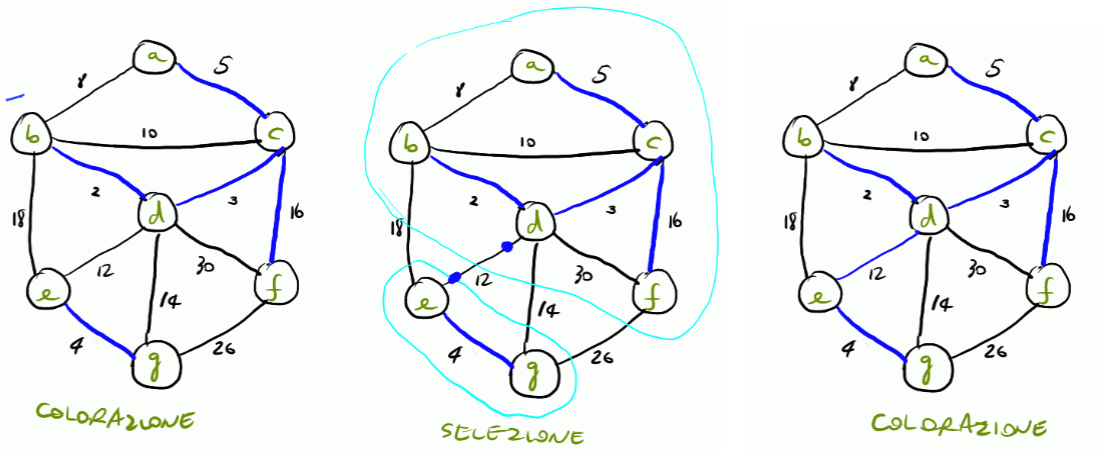
\includegraphics[width=0.5\linewidth]{Images/alberi_cammini_minimi/esempio_boruvka.png}
\end{figure}

\section{Algoritmo di Kruskal}
Seguendo un ordine crescente per costi di archi, se l'arco corrente e è contenuto in un albero blu\footnote{Cioè se l'arco considerato connette due nodi che sono già connessi nello stesso albero blu}, allora lo si colori di rosso, altrimenti lo si colori di blu.
\begin{figure}[H]
    \centering
    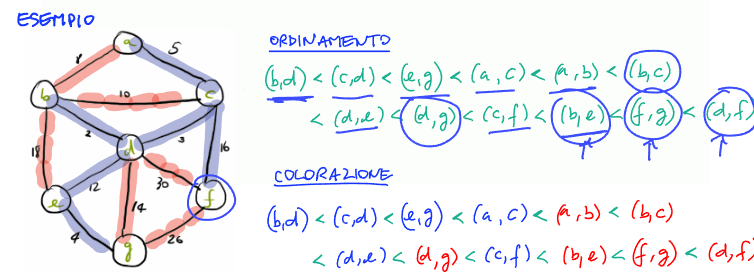
\includegraphics[width=0.5\linewidth]{Images/alberi_cammini_minimi/esempio_kruskal.png}
\end{figure}
Per dimostrare che questo algoritmo è corretto, procederemo per induzione:
\begin{itemize}
    \item \textbf{op($e_i$) colora $e_i$ di blu}: sia $e_i=(u_i, v_i)$, si ha che $u_i,v_i$ appartengono a due alberi distinti $S_i,T_i$\footnote{Altrimenti non potremmo colorarlo di blu}. Consideriamo il taglio $(S_i, V \backslash S_i)$, questo è attraversato dall'arco $e_i$ e, tutti gli archi $e:w(e)< w(e_i)$ sono già colorati a causa del funzionamento dell'algoritmo. Per cui, $e_i$ ha peso minimo tra tutti gli archi non colorati nel taglio, dunque può essere colorato di blu.
    \item \textbf{op($e_i$) colora $e_i$ di rosso}: sia $e_i=(u_i,v_i)$, $u_i, v_i$ appartengono allo stesso albero blu, sia $\pi$ il cammino da $u_i$ a $v_i$ in T, si consideri il ciclo $\pi_i;e_i$, tale ciclo non contiene archi rossi ed $e$ è l'unico arco non colorato, per cui possiamo fare un passo rosso.
\end{itemize}

Per gestire questo algoritmo, possiamo sfruttare ciò che abbiamo fatto con le strutture dati per insiemi disgiunti, ottenendo la seguente complessità:
\begin{figure}[H]
    \centering
    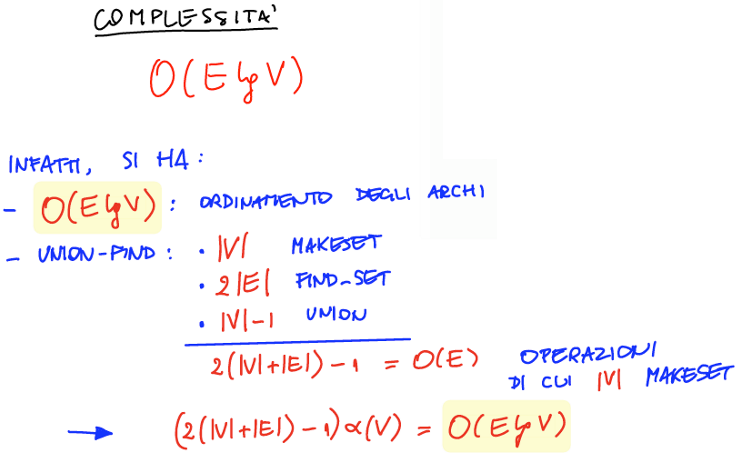
\includegraphics[width=0.6\linewidth]{Images/alberi_cammini_minimi/complessita_kruskal.png}
\end{figure}
\section{Algoritmo di Prim}
Passiamo, infine, all'algoritmo di Prim. Si seleziona un nodo s detto \textbf{sorgente} e si esegua per $|V|-1$ volte la seguente operazione:
\begin{itemize}
    \item si seleziona l'albero blu T contenente S.
    \item Si selezioni l'arco minimo incidente su T e lo si colori di blu.
\end{itemize}
In base a questo algoritmo possono esserci più MST in base alla sorgente da cui si parte. Tuttavia, se vale che la funzione peso è \textbf{iniettiva}, allora G ha un unico MST e ciò si può dimostrare nel seguente modo:
Siano $T_1 \neq T_2$ due MST di G, sia $(u,v) \in E[T_1]\backslash E[T_2]$, sia $\pi$ un cammino da u a v in $T_2$,ovviamente $\pi \nsubseteq T_1$. Sia 
\[(u',v') \in (E[T_2]\backslash E[T_1]) \cap \pi \subseteq E[T_1] \Delta E[T_2]\]
Pertanto $w(u',v') > w(u,v)$, sia $T_2' = T_2\{(u',v')\} \cup \{u,v\}$ si ha che $T'_2$ è un albero e $w(T_2') = w(T_2)-w(u',v')+w(u,v) < w(T_2)$ e ciò sarebbe assurdo perché abbiamo detto che $T_2$ è un MST. \\
Vediamo un esempio di esecuzione dell'algoritmo di Prim:
\begin{figure}[H]
    \centering
    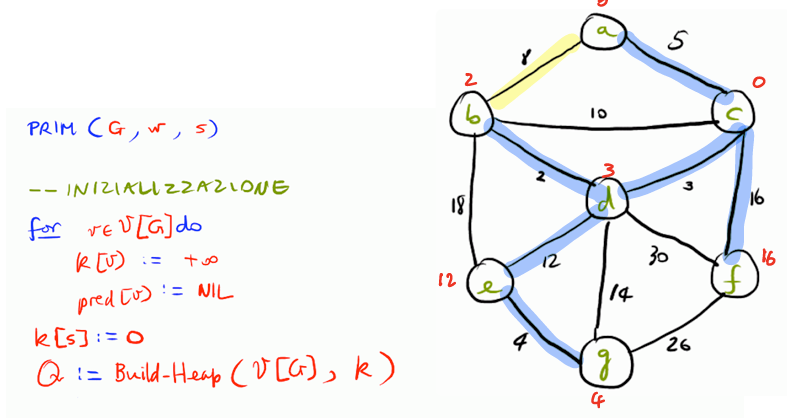
\includegraphics[width=0.7\linewidth]{Images/alberi_cammini_minimi/esempio_prim_1.png}
\end{figure}
\begin{figure}[H]
    \centering
    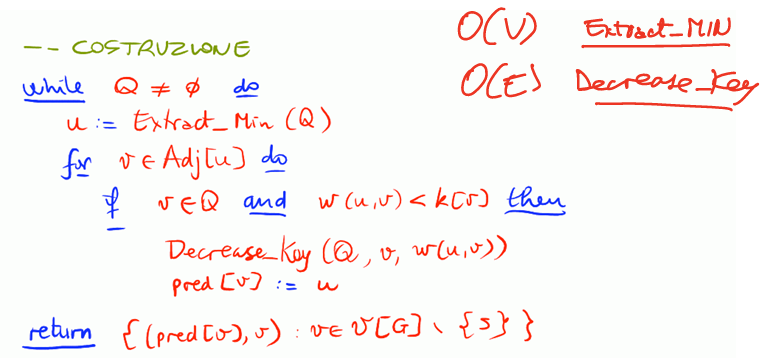
\includegraphics[width=0.7\linewidth]{Images/alberi_cammini_minimi/esempio_prim_2.png}
\end{figure}
Infine, diamo uno sguardo alla complessità di questo algoritmo, tenendo in considerazione le diverse implementazioni di Heap che abbiamo visto nei precedenti capitoli:
\begin{figure}[H]
    \centering
    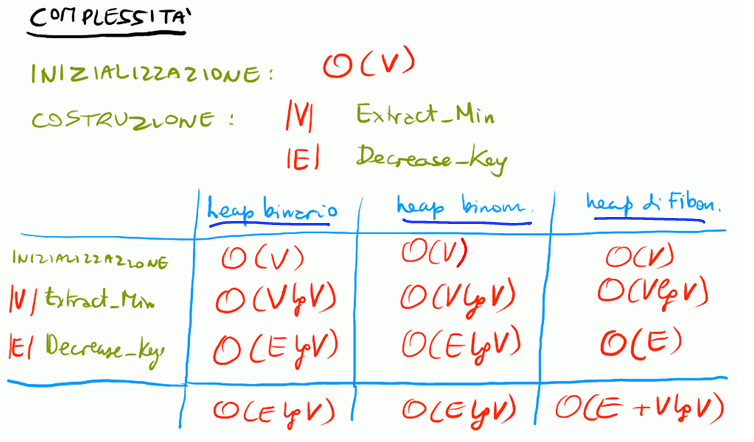
\includegraphics[width=0.6\linewidth]{Images/alberi_cammini_minimi/complessita_prim.png}
\end{figure}

\section{Signature di uno Spanning Tree}
Siano $r_1 = (V,T_1)$ e siano $r_2 = (V, T_2)$ due spanning di un medesimo grafo, definiamo \textbf{distanza tra $r_1$ e $r_2$} ponendo:
\[d(r_1,r_2) = d(T_1, T_2)=\frac{|T_1 \Delta T_2|}{2}\]

Sia $G=(V,E)$ un grafo non orientato con una funzione peso $w:E\rightarrow R $, la \textbf{segnatura} $\sum_w(G)$ di G è la sequenza dei pesi degli archi di G in ordine non decrescente:
\begin{figure}[H]
    \centering
    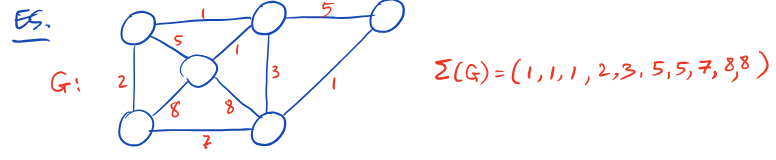
\includegraphics[width=0.6\linewidth]{Images/alberi_cammini_minimi/signature_esempio.png}
\end{figure}
Supponiamo adesso di prendere i seguenti MST e le relative signature:
\begin{figure}[H]
    \centering
    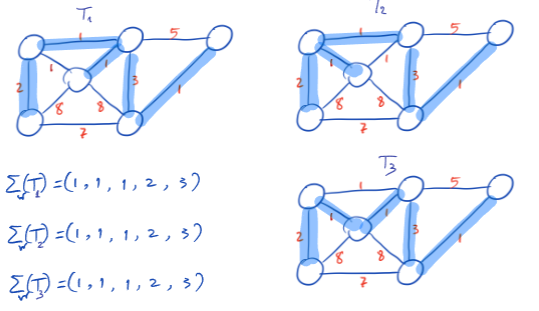
\includegraphics[width=0.6\linewidth]{Images/alberi_cammini_minimi/signature_mst.png}
\end{figure}
Come possiamo notare, tutte le signature di questi MST sono uguali.\\
\textbf{Teorema Unicità della signature di MST}\\
Due qualunque MST di uno stesso grafo pesato non orientato e connesso hanno la stessa segnatura.\\
Sia $(G,w)$ un grafo non orientato connesso e pesato contenente degli MST con signature diverse. In particolare, siano $r_1 = (V, T_1)$ e $r_2=(V, T_2)$ due MST con signature distinte tali che la loro distanza $d(T_1, T_2)$ sia minima. \\

Sia $e=(u,v)$ un arco di peso minimo in $T_1 \Delta T_2$\footnote{Cioè l'insieme composto dagli elementi univoci di entrambi gli insiemi}, e supponiamo che $e \in T_1$ e $e \notin T_2$.
Sia $(V_1,V_2)$ il taglio di G indotto cancellando dall'MST $r_1$ l'arco $e$. \\

Sia $\pi$ un cammino in $r_2$ da $u \in V_1$ a $v \in V_2$, e sia $e'$ un arco in $\pi$ che attraversa il taglio, allora $e' \in T_2 \backslash T_1$. Per la minimalità di $w(e)$ in $T_1 \Delta T_2$ si ha che $w(e) \leq w(e')$. Pertanto, posto $T_2' = (T_2 \backslash \{e'\}) \cup \{e\}$ si ha che $r'_2 = (V, T_2')$ è uno spanning tree di G, per cui:
\[w(T_2)\leq w(T'_2) = w(T_2)-w(e')+w(e)\leq w(T_2)\]
Da cui $w(T_2')=w(T_2)$ e, quindi, $r'_2 = (V,T_2')$ è un MST di G. Notiamo che:
\[\sum_w(r_2') = \sum_w (r_2) \neq \sum_w (r_1)\]
E quindi:
\begin{figure}[H]
    \centering
    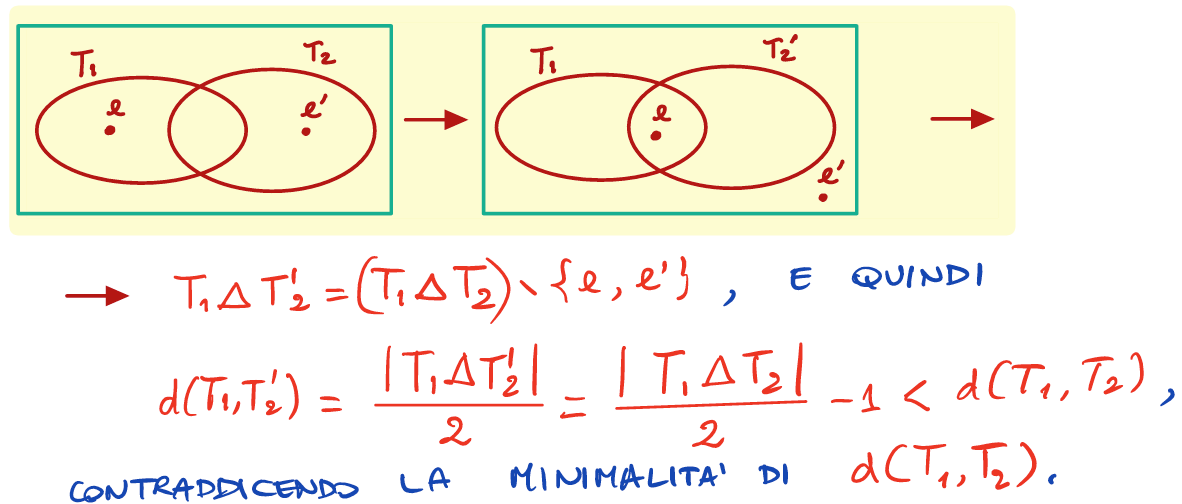
\includegraphics[width=0.7\linewidth]{Images/alberi_cammini_minimi/minimalita_distanza.png}
\end{figure}
\section{Minimalità della Signature di un MST}
Siano $\sigma = (s_1,\dots,s_k)$ e $\sigma' = (s_1',\dots,s_k')$ due k-uple di numeri reali, poniamo $ \sigma < \sigma'$ se $\sigma$ precede $\sigma'$ lessicograficamente, cioè:
\[s_1=s_1', s_2=s_2', \dots, s_{l-1}=s_{l-1}', s_l < s'_l\]
Queste relazioni godono delle seguenti proprietà:
\begin{itemize}
    \item La relazione di precedenza è \textbf{transitiva}.
    \item Sia $(G,w)$ un grafo non orientato pesato, con $G=(V,E)$ e sia $w':E\rightarrow R$ una qualunque funzione peso tale che:
        \begin{itemize}
            \item $w'(e)\leq w(e)$ per cui $e \in E$
            \item $w'(f)< w(f)$ per qualche $f \in E$\footnote{Cioè almeno un elemento deve essere diverso}
        \end{itemize}
\end{itemize}
Allora la segnatura di $(G,w')$ precede la segnatura di $(G,w)$.\\
\textbf{Teorema}\\
Uno spanning tree è un MST se e solo se la sua segnatura è \textbf{lessicograficamente minima}.\\
\textbf{Dimostrazione}\\
Supponiamo esista un grafo pesato $(G, w)$ non orientato e connesso con $G=(V,E)$ i cui MST hanno una segnatura $\sigma$ non minima. Siano $r,r'$ con $r=(V,T), r'=(V,T')$ una coppia di spanning tree tali che:
\begin{itemize}
    \item r sia un MST
    \item $\sigma'=\sum_w (r') < \sum_w (r) = \sigma$
    \item $d(r,r')$ sia minima
    \item $e \in T \Delta T'$ di peso minimo con $e = (u,v)$.
\end{itemize}
Distinguiamo adesso i due casi:
\begin{itemize}
    \item \textbf{$e \in T\backslash T'$}: Sia $(V_1, V_2)$ il taglio G indotto cancellando e dall'MST $r$. Sia $\pi$ un cammino $r'$ da u a v e sia $e'$ un arco in $\pi$ che attraversa il taglio. Allora $w(e) \leq w(e')$. Poiché $(T' \backslash \{e'\} \cup \{e\})$ è uno spanning tree, si ha che:
    \[\sum_w(T' \backslash \{e'\} \cup \{e\} ) \leq \sum_w(T') < \sum_w(T)\]
    Inoltre:
    \[d((T' \backslash \{e'\} \cup \{e\}),T) < d(T',T)\]
    E ciò contraddice la minimalità di $d(T',T)$.
    \item \textbf{$e \in T'\backslash T$}: Sia $(V_1, V_2)$ il taglio G indotto cancellando dallo spanning tree $r'$. Sia $\pi$ un cammino in $r$ da u a v e sia $e'$ un arco in $\pi$ che attraversa il taglio, allora $e' \in T \backslash T'$. Al solito, $(T \backslash \{e'\})\cup \{e\}$ è uno spanning tree di $G=(V, E)$. Poiché $w(e) \leq w(e')$ si ha che:
    \[w(T)\leq w((T \backslash \{e'\})\cup \{e\})\leq w(T)\]
    Dunque: $\sum_w(T') < \sum_w(T) = \sum_w((T \backslash \{e'\})\cup \{e\})$, inoltre $d(T', (T \backslash \{e'\})\cup \{e\}) < d(T',T)$ e ciò contraddice la minimalità di $d(T',T)$.
\end{itemize}
Dimostriamo adesso il viceversa.\\
Sia $r$ uno spanning tree con segnatura minima e sia $r'$ un mst di G. Per la prima parte del teorema $r'$ è minima, dunque $\sum_w (r) = \sum_w(r')$ da cui si dimostra banalmente che anche $r$ è un mst.

\section{Clustering}
Supponiamo di avere una collezione di oggetti che è necessario inserire in dei gruppi di oggetti simili. È necessario avere una \textbf{funzione distanza} tra gli oggetti in modo da avere un grado di somiglianza tra questi.
Il problema del \textbf{clustering} è il problema di suddividere opportunamente un dato insieme di oggetti in modo tale che oggetti vicini in termini della funzione distanza stabilita, appartengano allo stesso cluster e oggetti lontani a cluster diversi.

Per fare ciò, sfruttiamo l'algoritmo di Kruskal precedentemente mostrato. Grazie a questo si ricercano cluster che assicurino la massima distanza tra ciascuna coppia di cluster distinti.

Sia $U = \{p_1, p_2, \dots, p_n\}$ un insieme di oggetti dotato di una funzione distanza $d:U \times U \rightarrow R$ tale che:
\begin{itemize}
    \item $d(p_i,p_i)=0$ per ogni $i=1,\dots , n$
    \item $d(p_i,p_j)>0$ per ogni $1\leq i,j \leq n$
    \item $d(p_i,p_j) = d(p_j,p_i)$ per ogni $1\leq i,j \leq n$.
\end{itemize}
Sia fissato $k \leq n$ assegnato e chiamato \textbf{numero di cluster}. Una partizione $C_1, C_2, \dots, C_k$ di $U$ tale che $c_i \neq 0$ per ogni $i=1,\dots, k$, questa è detta $k-clustering$ di $U$. 
Dato un $k-clustering$ $C=\{C_1, C_2, \dots, C_k\}$ di $U$, la \textbf{separazione di C} è data da:
\begin{align*}
    &d(C_i,C_j) = \min d(p,q) : p\in C_i, q \in C_j \quad \text{Distanza tra due cluster}\\
    &sep(C) = \min_{i\neq j}d(C_i,C_j) \quad \text{Grado di separazione di C}
\end{align*}

Dato un insieme U con funzione d e un intero k, definiamo il problema del \textbf{$k-clustering$ a separazione massima per $(U, d)$} il problema di trovare un $k-clustering$ C di U tale che:
\[sep(C)\geq sep(C')\]
Per ogni altro $k-clustering$ $C'$ di U.

\subsection{Algoritmo di Kruskal Clustering}
Dopo avere effettuato opportune modifiche, tramite l'algoritmo di Kruskal è possibile risolvere il problema del clustering a separazione massima.
\begin{figure}[H]
    \centering
    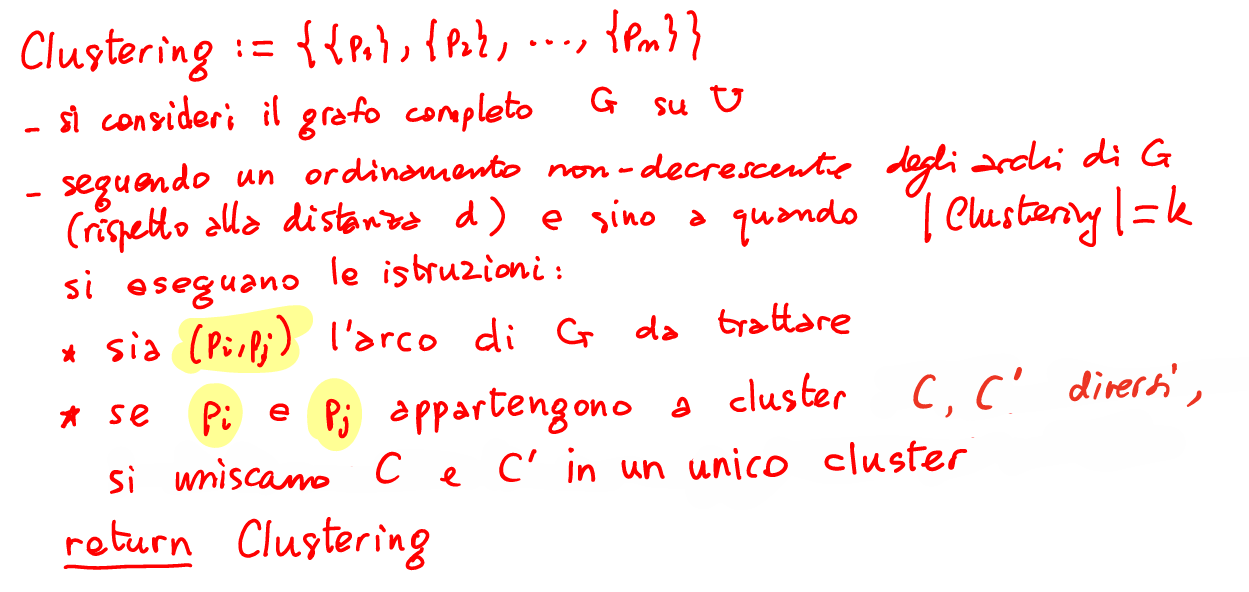
\includegraphics[width=0.7\linewidth]{Images/alberi_cammini_minimi/clustering/algoritmo_kruskal.png}
\end{figure}
In pratica, le modifiche che abbiamo effettuato sono: 
\begin{itemize}
    \item L'algoritmo si ferma quando il numero di alberi della foresta è $k$ e non 1.
    \item L'algoritmo restituisce le componenti connesse della foresta trovata.
\end{itemize}
La complessità di questo algoritmo è $O(n^2log(n))$.
Possiamo osservare che la separazione del cluster così calcolato è maggiore o uguale al peso $d(p_i,p_j)$ dell'arco $(p_i,p_j)$ che l'algoritmo avrebbe preso in considerazione se non si fosse fermato.
Ciò è dovuto al fatto che l'algoritmo si è fermato prima di aggiungere quest'ultimo arco e, quindi, tutti gli archi prima di lui sono più corti. Consideriamo adesso due punti p e q che sono in cluster diversi e che definiscono la separazione, l'arco tra di loro non può essere già stato processato, altrimenti p e q sarebbero nello stesso cluster e, se questo arco non è ancora stato processato, deve essere perché la sua lunghezza è almeno uguale a quella del prossimo arco in lista. Dunque, deve per forza essere che $sep(C) \geq d(p_i,p_j)$.\\
\textbf{Correttezza dell'algoritmo}\\
Sia $C*=\{C_1, \dots, C_k\}$ il $k-clustering$ costruito dall'algoritmo. Come osservato prima $sep(C*)\geq d*$ dove $d*$ è il peso dell'arco che sarebbe stato preso in considerazione all'iterazione successiva. Sia $C'=\{C'_1, \dots, C'_2\}$ un qualunque altro clustering distinto da $C*$, dobbiamo verificare che $sep(C') \leq sep(C*)$.
Dato che $C* \neq C'$, almeno un cluster di $C*$ ne interseca due distinti di $C'$.
Sia $C_r \in C*$ tale che $C_r$ interseca due cluster distinti di $C'$:
\begin{itemize}
    \item Sia $p \in C_r$ e sia $C'_s \in C'$ tale che $p \in C'_s$. Cioè $p$ p è l'elemento contenuto in entrambi.
    \item Sia $q \in C_r$ tale che $q \notin C'_s$. Cioè q è contenuto solo in $C_r$.
\end{itemize}
Poiché p,q stanno nello stesso cluster $C_r$, essi sono connessi nel grafo da un cammino $\pi$ i cui archi hanno peso $\leq d*$. Quindi su $\pi$ vi sono due nodi contigui $p',p''$ tali che $p'\in C'_s, p'' \notin C'_s$, ma $d(p',p'')\leq d*$ e, quindi, $sep(C')\leq d* \leq sep(C*)$ da cui la tesi.
\begin{figure}[H]
    \centering
    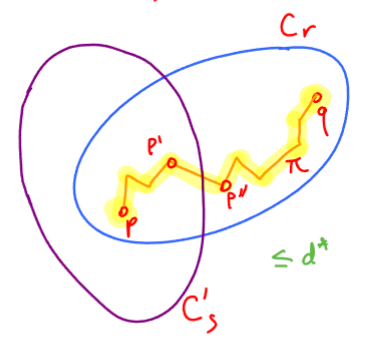
\includegraphics[width=0.4\linewidth]{Images/alberi_cammini_minimi/clustering/dimostrazione_correttezza.png}
\end{figure}

\subsection{Minimum Spanning Tree in Grafi Sparsi}
Definiamo una \textbf{contrazione} di un grafo \textbf{non orientato} $G=(V,E)$ un grafo $G'=(V',E')$ tale che:
\begin{itemize}
    \item $V'=\{V_1,V_2,\dots ,V_k \}$ è una partizione di V. \footnote{Raggruppiamo i nodi in gruppi.}
    \item Ogni sottografo di $G=(V,E)$ indotto dagli insiemi di vertici $V_1,V_2,\dots ,V_k$ è connesso. \footnote{In ogni gruppo i nodi devono essere connessi.}
    \item Per ogni coppia $v_i, v_j \in V'$ con $i \neq j$ si ha che: \footnote{Ogni gruppo è connesso se esiste un arco da un nodo di uno a uno dell'altro.}
    \[(v_i,v_j) \in E' \leftrightarrow (\exists v_i \in V_i, v_j\in V_j):(v_i,v_j)\in E\] 
    \begin{figure}[H]
        \centering
        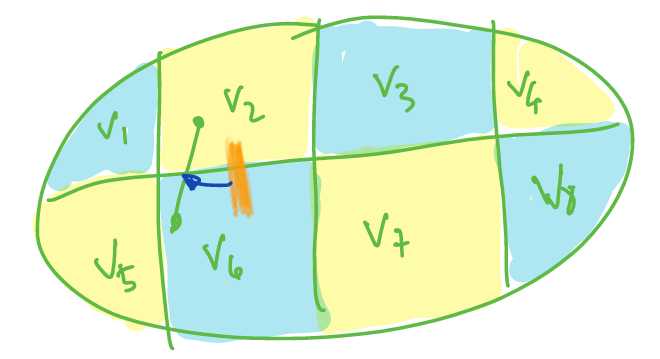
\includegraphics[width=0.4\linewidth]{Images/alberi_cammini_minimi/contrazione.png}
    \end{figure}
\end{itemize}
Dato un grafo non orientato e connesso $G=(V,E)$ con funzione peso $w:E \rightarrow R$, descriveremo una procedure \textbf{MST-Reduce} che costruisce:
\begin{itemize}
    \item Un grafo \textbf{contratto} $G'=(V',E')$ di $G=(V,E)$ con funzione peso $w':E' \rightarrow R$ dove $V'$ è una partizione di V tale che $|V'| \leq |V|/2$.\footnote{Ogni partizione ha al più la metà dei nodi originali}
    \item Una \textbf{funzione} $orig':E'\rightarrow E$ tale che:\footnote{Ogni arco nella che collega due partizioni, è un arco reale del grafo iniziale.}
    \[(u',v')\in E',orig'(u',v')=(u,v)\rightarrow (u\in u',v \in v',w'(u',v')=w(u,v))\]
    \item Un insieme di archi $T \subseteq E$ tale che:
    \[(\forall (u_1,u_2)\in T) (\exists V_i \in V'): u_1,u_2 \in V_i\]
    tali che per ogni \textbf{MST} $a$ di $(G',w')$:\footnote{Gli archi in $T$ sono quelli che sono finiti dentro i supernodi. Siccome li abbiamo usati per la contrazione, siamo sicuri che facciano parte della soluzione ottimale }
    \[T \cup orig'[a] \text{ è un MST di $(G,w)$}\]
\end{itemize}
Gli archi di $T$ che si trovano "dentro" il gruppo $V_i$ formano l'Albero di Copertura Minimo (MST) del sottografo indotto dai vertici di $V_i$.
\begin{figure}[H]
    \centering
    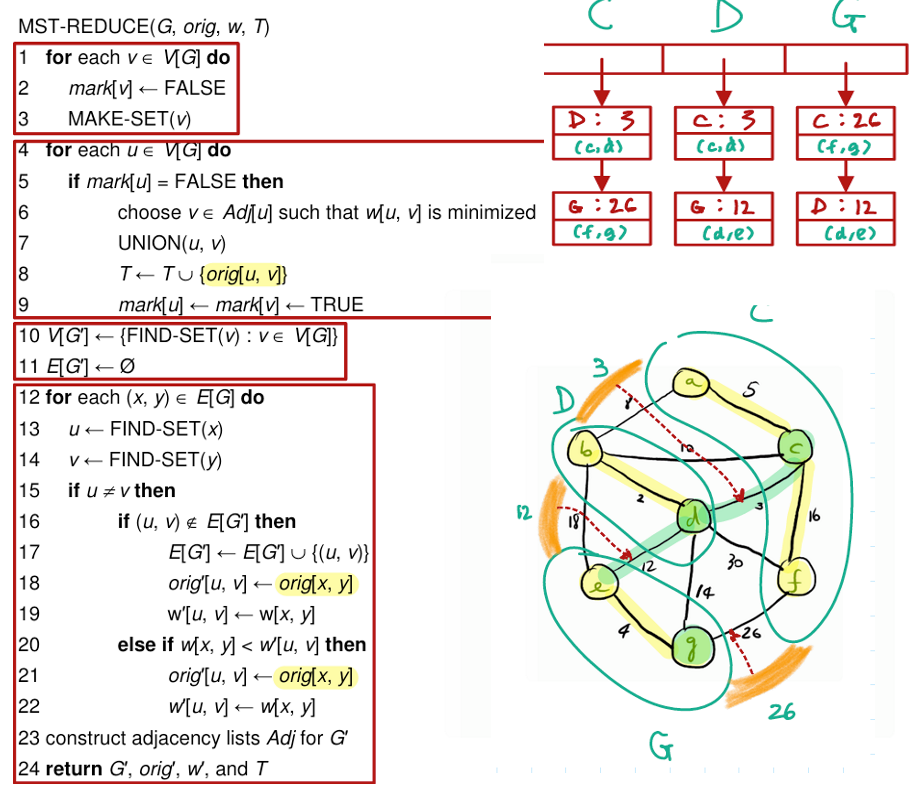
\includegraphics[width=0.9\linewidth]{Images/alberi_cammini_minimi/mst_reduce.png}
\end{figure}
L'algoritmo si compone di varie fasi:
\begin{enumerate}
    \item All'inizio ogni nodo è da solo (interpretato come insieme a se' stante) e viene marcato come FALSE.
    \item L'algoritmo scorre tutti i nodi. Se trova un nodo u che non è ancora stato toccato (cioè marcato con FALSE) allora si cerca l'arco più leggero che parte da u e arriva a v e si fondono i due gruppi e marca u e v come true.
    \item I nuovi nodi non sono altro che i "rappresentanti" (trovati con FIND-SET) dei gruppi che abbiamo creato prima. Se abbiamo unito $A, B, C$, il nuovo nodo sarà il nome del rappresentante di quel gruppo.
    \item L'algoritmo scorre tutti gli archi originali $(x, y)$ del grafo vecchio e per ogni arco, guarda a quale "regione" appartengono gli estremi e se la regione di partenza è diversa, controlliamo due casi: 
        \begin{itemize}
            \item Caso 1: Se non c'è ancora un arco tra la Regione $u$ e la Regione $v$ nel nuovo grafo, lo creiamo usando il peso dell'arco $(x, y)$.
            \item Caso 2: Se esiste già un arco tra $u$ e $v$, controlliamo il peso e teniamo solo quello minore.
        \end{itemize}
    \item Infine, costruiamo la lista di adiacenza per $G'$. 
\end{enumerate}

